\documentclass[12pt]{article}

\usepackage{answers}
\usepackage{setspace}
\usepackage{graphicx}
\usepackage{enumitem}
\usepackage{multicol}
\usepackage{mathrsfs}
\usepackage[margin=1in]{geometry} 
\usepackage{amsmath,amsthm,amssymb}
\usepackage[english]{babel}

\newcommand{\N}{\mathbb{N}}
\newcommand{\Z}{\mathbb{Z}}
\newcommand{\C}{\mathbb{C}}
\newcommand{\R}{\mathbb{R}}

\DeclareMathOperator{\sech}{sech}
\DeclareMathOperator{\csch}{csch}

\newenvironment{theorem}[2][Theorem]{\begin{trivlist}
		\item[\hskip \labelsep {\bfseries #1}\hskip \labelsep {\bfseries #2.}]}{\end{trivlist}}
\newenvironment{definition}[2][Definition]{\begin{trivlist}
		\item[\hskip \labelsep {\bfseries #1}\hskip \labelsep {\bfseries #2.}]}{\end{trivlist}}
\newenvironment{proposition}[2][Proposition]{\begin{trivlist}
		\item[\hskip \labelsep {\bfseries #1}\hskip \labelsep {\bfseries #2.}]}{\end{trivlist}}
\newenvironment{lemma}[2][Lemma]{\begin{trivlist}
		\item[\hskip \labelsep {\bfseries #1}\hskip \labelsep {\bfseries #2.}]}{\end{trivlist}}
\newenvironment{exercise}[2][Exercise]{\begin{trivlist}
		\item[\hskip \labelsep {\bfseries #1}\hskip \labelsep {\bfseries #2.}]}{\end{trivlist}}
\newenvironment{solution}[2][Solution]{\begin{trivlist}
		\item[\hskip \labelsep {\bfseries #1}]}{\end{trivlist}}
\newenvironment{problem}[2][Problem]{\begin{trivlist}
		\item[\hskip \labelsep {\bfseries #1}\hskip \labelsep {\bfseries #2.}]}{\end{trivlist}}
\newenvironment{question}[2][Question]{\begin{trivlist}
		\item[\hskip \labelsep {\bfseries #1}\hskip \labelsep {\bfseries #2.}]}{\end{trivlist}}
\newenvironment{corollary}[2][Corollary]{\begin{trivlist}
		\item[\hskip \labelsep {\bfseries #1}\hskip \labelsep {\bfseries #2.}]}{\end{trivlist}}

\begin{document}
	
	% --------------------------------------------------------------
	%                         Start here
	% --------------------------------------------------------------
	
	\title{IT-Security}%replace with the appropriate homework number
	\author{Michael Gabler} %if necessary, replace with your course title
	
	\maketitle
	
	\section{Definitions}
	
	\textbf{C-I-A Triad}
	\begin{enumerate}
		\item \textbf{C}onfidentiality: prevents unauthorized access to private data
		\item \textbf{I}ntegrity: protects information from being modified by unauthorized parties
		\item \textbf{A}vailability: authorized parties have access to the information when needed
		\item \textbf{A}uthenticity: Being able to verify a party
		\item \textbf{A}ccountability: To guaranty that a property or action belongs to one specific entity
	\end{enumerate}
	\textbf{Security Threat} A potential for violation of security (interruption (a), interception (p), modification (a), fabrication (a) of information) $\rightarrow$ splits up into active and passive\\
	\textbf{Security Attack} Action that compromises the security of information\\
	\textbf{Security Mechanism} A process or device that is designed to detect, prevent or recover from a security attack\\
	\textbf{Security Service} Service to prevent security attacks by implementing one or more mechanisms
	
	\section{Cryptography}
	\textbf{Kerckhoffs' principle} \textit{The enemy knows the system} $\rightarrow$ The cipher should remain secure if the adversary knows the specification of the cipher\\
	$\Rightarrow$ not respecting this principle means \textbf{security by obscurity}\\
	\textbf{Encryption Scheme} is a pair of encryption ($Enc$) and decryption ($Dec$) algorithm with $Dec_k(Enc_k(m)) = m$ for every plaintext message $m \in M$ plaintext space and key $k \in K$ key space. $Dec_k(m) = c$ generates the cipher $c \in C$ ciphertext space.\\
	\textbf{Security of an encryption scheme} The adversary should not learn any additional information about $m$ when receiving $c$
	
	\subsection{Historical ciphers}
	\paragraph{Caesar's shift cipher} $M = {A,...,Z} = {0,...,25}$ words over alphabet\\
	$K = {0,...25}$\\
	$Enc_k(m_0,...,m_n) = (k+m_0 mod 26,..., k+m_n mod 26)$\\
	$Dec_k(c_0,...,c_n) = (c_0-k mod 26,..., c_n-k mod 26)$\\
	$\Rightarrow$ can be broken by brute force attack (try every key) since $|K| = 26$
	\paragraph{Substitution cipher}
	Do not shift each letter with the same key but use a mapping table\\
	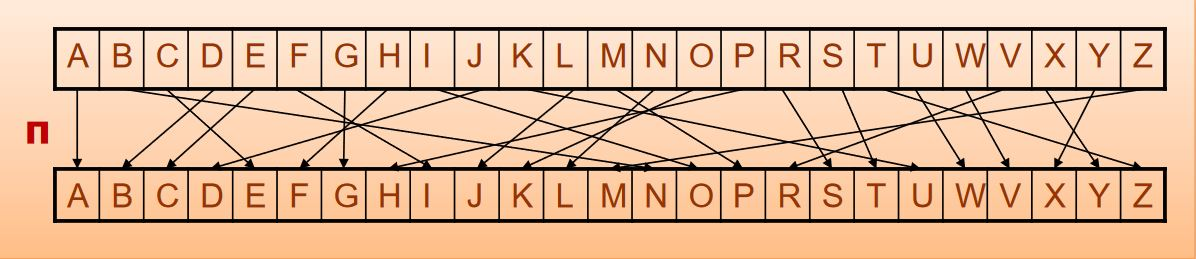
\includegraphics[width=\textwidth]{figures/substitution-cipher.JPG}\\
	$\Rightarrow$ can be broken by using statistical patterns: for example the letter E is the most frequent in the german language
	\paragraph{Vigenère cipher} Use a key with arbitrary length of letters. Each letter of the key defines the shift value for a plaintext letter. If the plaintext is longer than the key it must be repeated.\\
	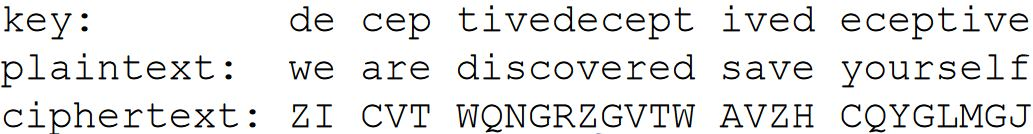
\includegraphics[width=\textwidth]{figures/vigenere-cipher.JPG}\\
	$\Rightarrow$ when the key is repeated its possible that the same letters are encrypted with the same shift which result in the same ciphertext. If such \textbf{identical parts} are found the \textbf{length of $k$} can be computed. Now it's possible to break the cipher by applying $|k|$-times the \textbf{frequency attack} from the substitution cipher.
	
	\subsection{One-time pad}
	$K = M = C = {0,1}^t$\\
	$Enc_k(m) = k xor m$\\
	$Dec_k(m) = k xor c$\\
	$\Rightarrow$ This is perfectly secure but not practical because a key can only be used once (otherwise same ciphertext for same plaintext) and therefore must be as long as the message which is also not practical. So there's no other perfectly secret cipher.\\
	$\Rightarrow$ Other encryption sche\\mes rely on a limitation of the adversary's power (mostly meant \underline{computational} power)
	\textbf{Computational security} A system $X$ is $(t,\epsilon)$-secure if every Turing Machine that operates in time $t$ can break it with probability at most $\epsilon$ where $\epsilon$ is negligible (close to 0).
	
	\subsection{Attacks}
	\textbf{Ciphertext-only attack} The adversary has no information about the plaintext\\
	\textbf{Known plaintext attack} The plaintext is drawn from some distribution that the adversary does not control\\
	\textbf{Chosen-plaintext attack} The adversary can choose arbitrary plaintext and receives the ciphertext from it\\
	\textbf{Chosen-ciphertext attack} The adversary gets information by receiving the decryption of chosen ciphertexts
	
	\subsection{Modern cryptography}
	\textbf{One-way functions} are functions that are poly-time computable and hard to invert. Rely on a mathematical hardness assumption.\\
	\textbf{Pseudorandom generators (PRG)} Generate bits that look random. Depens on a seed (for example system time). Can be constructed by using a one-way function. They are cryptographic if it's not % TODO finish definition\\
	\textbf{Stream cipher} cipher with an infinite stream of bits as output (for example RC4 used for WEP, WPA) $\rightarrow$ PRGs are stream ciphers\\
	\textbf{Block ciphers} % TODO continue with slide 47, presentation 03
	

	
	
\end{document}
